\section{Figures} % (fold)
\label{sec:list_of_figures}


\begin{figure}[h]
    \centering
    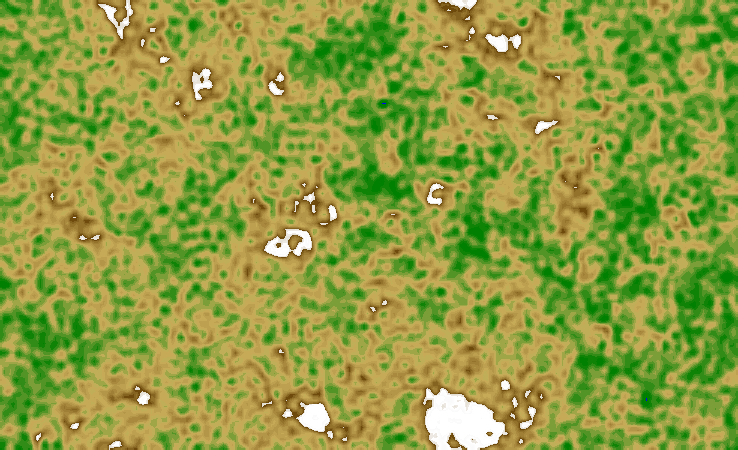
\includegraphics[angle=90, width=0.6\textwidth]{figures/map.jpg}
    \caption{U-matrix visualisation of the SOM, after training with 10.000 songs}
    \label{fig:map}
\end{figure}

\begin{figure}[h]
    \centering
    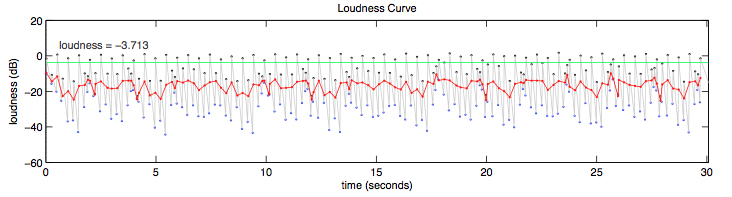
\includegraphics[width=\textwidth]{figures/loudness.jpg}
    \caption{Graphical representation of the loudness attributes of the segments from 39 seconds of "Around The World" by Daft Punk.}
    \label{fig:loudness}
\end{figure}

\begin{figure}[h]
    \centering
    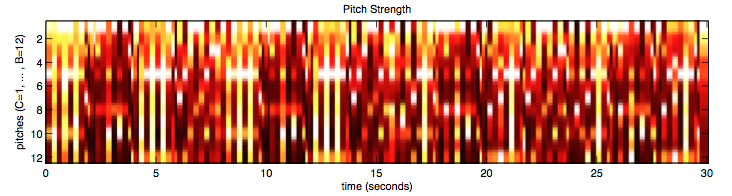
\includegraphics[width=\textwidth]{figures/pitch.jpg}
    \caption{Graphical representation of the ptich vector attributes of the segments from 39 seconds of "Around The World" by Daft Punk.}
    \label{fig:pitch}
\end{figure}

\begin{figure}[h]
    \centering
    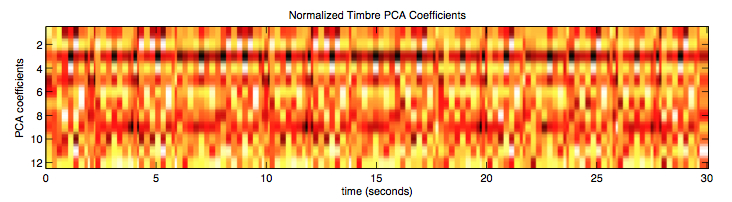
\includegraphics[width=\textwidth]{figures/timbre.jpg}
    \caption{Graphical representation of the timbre vector attributes of the segments from 39 seconds of "Around The World" by Daft Punk.}
    \label{fig:timbre}
\end{figure}


\begin{figure}[h]
    \centering
    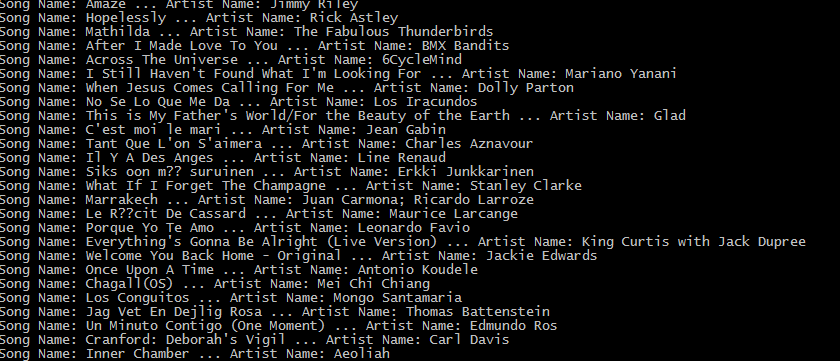
\includegraphics[width=\textwidth]{figures/ESOMSongs.PNG}
    \caption{Playlist description with ESOM path generation}
    \label{fig:esomres}
\end{figure}

\begin{figure}[h]
    \centering
    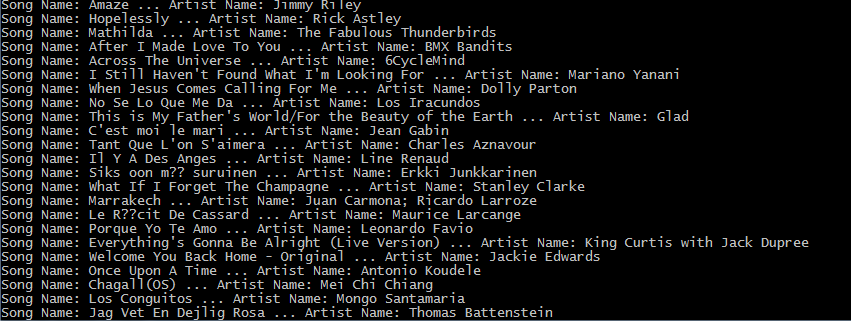
\includegraphics[width=\textwidth]{figures/UMatSongs.PNG}
    \caption{Playlist description with UMat path generation}
    \label{fig:umatres}
\end{figure}


% section list_of_figures (end)